%%Introduction

%%State the objectives of the work and provide an adequate background, avoiding a detailed literature survey or a summary of the results.

%The advent of computer Aid design paired with the already established industrialization of construction, brought in during the creation of the rationalism movement on the 20th century, has provoked a new paradigm shift in the architecture design. The cult of the oversimplification and the ideas of functionality brought by their most canonical representative "Le Corbusier" that birthed cities alienated from the human centric design that had created urban spaces and society \cite{Stacbond2020} in favor for minimalistic approches following an industrial design that ppointed to the machine as the new model for building design \cite{Economakis2023}

%I want to describe the opportunity to bring back ornament and identity to the urban space and buildings by the integration of digital fabrication. as a response to the one size fits all state of current building design that stills considers above all eficiency.

%Also do a quick timeline of the progress of styles or evolution of paradigm in architecture throughout history with the purpose of showing how simplicity follows complexity and how society responds in a bit of a cyclical way to it.

%talk about biomimetics too since might be a comunion between performance and aesthetics while contextualizing architecture.

%mention the oportunity of mixed reality to convey all this information to the stakeholders so that they can feel the advantages of great design with the empowering tools of digital fabrication that could reshape the very understanding of common construction with the soon to come democratization of 3d printing houses and other digital fabrication techniques.

%%%%%% Start of text

The emergence of computer-aided design and digital fabrication could herald a resurgence of intricate and ornate architectural design within our societal fabric, potentially offering a remedy to the uniformity plaguing today's urban landscapes.

This research aims to explore the user response to complex facades created with digital fabrication, measured through a mixed reality experiment, to Refine our understanding of complex Facade Design and investigate the possible correlations between these insights and predictions of Future Construction Trends.

Upon delving into the annals of influential architectural styles, a discernible pattern emerges—an oscillation between simplicity and complexity(see Figure \ref{fig:TimelineArchitecture}). This recurrent cycle in architectural paradigms is not only reflective of the values ingrained in the societies they house, but also closely tied to pivotal technological advancements.

%% Timeline Architecture Image
     \begin{figure}[htb]
          \centering
          % trim=left 190 down 250 right 150 top5
          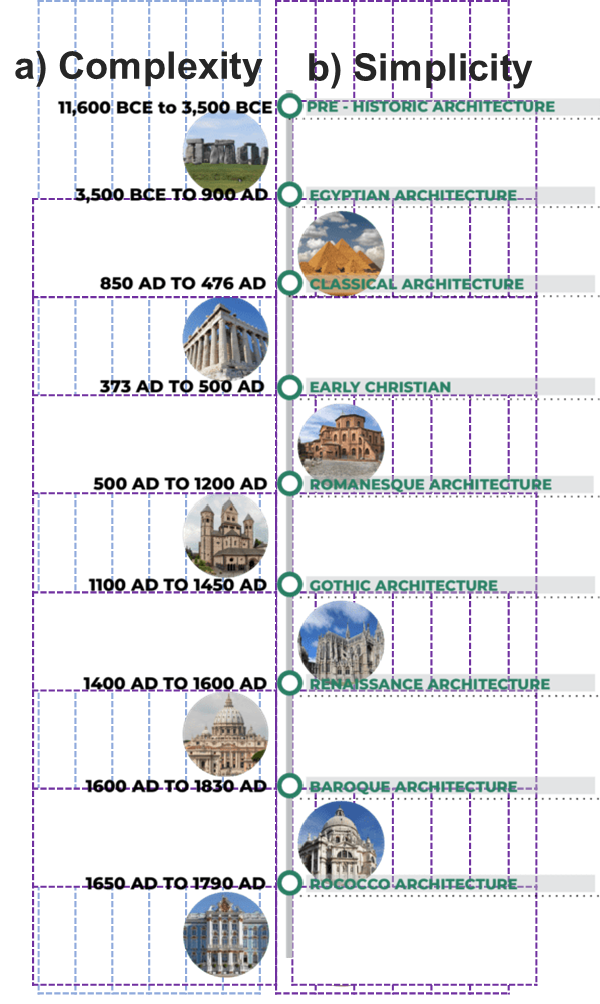
\includegraphics[width= \linewidth]{Images/TimelineArchitecture.pdf}
          \caption{Timeline of Architecture and the recurrent pattern of complexity and simplicity}
          \label{fig:TimelineArchitecture}
        \end{figure}

Consider, for instance, the transition from the robust Romanesque classic style of the 10th century, notably exhibited in churches \cite{Arora2023}, to the groundbreaking advancements of the 12th century that introduced buttresses, revolutionizing load distribution. This innovation propelled churches skyward, inviting luminous interplays to embellish the interiors with stunning stained-glass windows bedecked in intricate designs \cite{Stacbond2020}.

This trend resurfaced as time unfolded, transitioning from the complex Gothic style to the revival of Greek and Roman ideals, exemplified by the symmetrical perfection of the Renaissance era in the 14th century. This resurgence was succeeded by the opulent ornamentation of the Baroque style in the 16th century, followed by the neoclassical revival of the 18th century, heavily influenced by classical Greek and Palladian architecture. In the 1920s and 30s, the intricate Art Deco movement emerged, celebrating technological progress through luxurious materials and patterns seamlessly integrated with modern design and manufacturing techniques.

In response to this progression, the first half of the 20th century witnessed the emergence of Modern Architecture and rationalism. This architectural ethos adopted the maxim "Form follows function" \cite{Gage2015}, emphasizing functionalism and minimalistic architecture that showcased new-age materials such as steel, glass, and concrete \cite{Arora2023}.

TThis shift encapsulates the quintessence of architectural evolution—an ever-changing interplay between simplicity and complexity, often steered by the confluence of societal values and technological breakthroughs.

Once again, we find ourselves at a pivotal juncture in history, as the emergence of computer-aided design converges with the industrialization of construction, ushering in a new paradigm in architectural design. The 20th-century dominance of Rationalism, exemplified by figures like Le Corbusier, underscored an ethos of oversimplification and functionality. Characterized by straightforward, symmetrical forms and concrete as the favored medium, this era yielded cities estranged from human-centric design. Swift transportation took precedence, fracturing urban spaces that once defined vibrant societies \cite{Stacbond2020}. Subsequently, industrial design asserted its dominance as the blueprint for future construction \cite{Economakis2023}, casting architecture in the mold of minimalism and mass-produced uniformity, forsaking the ornate allure and individuality of yesteryears.

In response to the prevailing state of monotonous, one-size-fits-all building design, this paper embarks on an exploration—a quest to reintroduce ornamentation and identity to our urban spaces by embracing the fusion of digital fabrication. By harnessing the limitless potential of digital fabrication technology, architecture can rise above the constraints of mass production and rediscover its intricate and inspiring origins, while ensuring that the results remain compelling and well-received by users.

Amidst this transformative pursuit, the advent of mixed reality technology offers a portal to vividly convey the vision of future architectural design. Immersing stakeholders in a virtual realm where digital fabrication converges with artistry and functionality, we sow the seeds of a shared understanding of the virtues of complexity. Through this immersive experience, stakeholders bear witness to the rebirth of conventional construction methods, especially as the democratization of 3D printing houses and other digital fabrication techniques looms on the horizon.

Hence, this study sets out to address a pivotal question: What degree of complexity and pattern arrangement within facade design, generated through a data-driven design process tailored for digital fabrication, would users tolerate and accept for a building? Our hypothesis posits that regardless of participants' professional backgrounds and preexisting knowledge of facade design, their engagement in a Mixed Reality experiment (MR) would furnish the essential data required to refine our comprehension of complex facade design. Moreover, this data would lay the foundation for forecasting whether the shift towards intricate ornamentation will indeed shape the future trends of construction, as evidenced by the configurations they contribute. By embracing complexity and releasing the shackles of mass-produced uniformity, we embrace an opportunity to breathe new vitality into our urban realms, rekindle the essence of ornamentation and identity, and embrace an aesthetic sustainability inspired by the brilliance of the natural world.



        
%I want to include more references on the timeline
% add the concept of Object-Oriented. Using these concepts as basis. I want to express that the mr experiment is based on the idea that architecture as a tool should be invisible and confortable while in use. But it should  create emotion when seen as part of the landscape as a form of art to recapture the humand oriented city .

Heideggers tool analysis states that as the tool is a tool it dissapears in favor of some purpose he continues to explain that generally we don't notice equipment until it fails, like when An earthquake calls attention to the ground we walk or when a medical problem alerts us of the presence of organs that we have silently depended\cite{Harman2011}.
Harmans, Object-oriented ontology, borrows this concept to formulate its central claim that objects have hidden qualities and realities, and they withdraw from our understanding.\cite{Gage2015}
he idea that we live our lives on a layer of invisible equipment has significant ramifications for architecture, a discipline that produces the equipment on and in which we exist.\cite{Gage2015}

               %Traditionally, it was used to describe the impor- tance of a building revealing its structural system (the form  follows the function of the structure

               %The  idea that we live our lives on a layer of invisible equipment  has significant ramifications for architecture, a discipline that  produces the equipment on and in which we exist.

               %Heidegger's tool analysis posits that while a tool is func- tioning, or its function is visible, the mind registers it as  equipment and, as such, it is rendered invisible to our atten- tion

               %philosophical realism , that is, the belief that there  is a reality outside of the mind, as opposed to philosophical  idealism , which holds that reality exists primarily as a mental  construct.

                %A reaction against 20th-century continental  anti-realism , object-oriented ontology (OOO
